\documentclass{standalone}
\usepackage[dvipsnames]{xcolor}% set color
\usepackage{tikz}
\usetikzlibrary{cd} 
\usetikzlibrary{babel}
\usetikzlibrary {decorations.markings} % add marks on lines
\usetikzlibrary{decorations.pathmorphing} % wiggy lines 

\begin{document}
	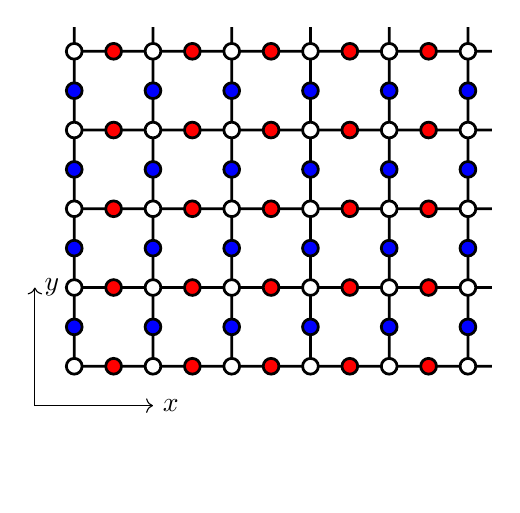
\begin{tikzpicture}
				[grid lines/.style= very thin,
		my grid/.style={grid lines, color=#1!50},
		my grid/.default=blue,
		circle A/.style={fill=white, radius=0.1},
		circle B/.style={fill=red, radius=0.1},
		circle C/.style={fill=blue, radius=0.1}]
		
		\def \Gx {1};
		\def \Gy {1};
		\def \ratio {1cm/1pt};
		
		\draw[->] (-3.5,-2.5) -- (-2,-2.5) node[right]{$x$};	
		\draw[->] (-3.5,-2.5) -- (-3.5,-1) node[right]{$y$};	
		% \draw[my grid] (-5, -5) grid (5,5);
		
		\clip (-3.5,-3.5) rectangle (2.3,2.3);
		\foreach \n in {-3, ..., 2}
			\foreach \m in {-2, ..., 2}
				{\begin{scope}[transparency group, xshift=\n*\Gx*\ratio, yshift=\m*\Gy*\ratio]
					\draw[] (0,0) -- (0,1);
					\draw[] (0,0) -- (1, 0);
					\draw[circle A] (0,0) circle;
					\draw[circle B] (1/2,0) circle;
					\draw[circle C] (0,1/2) circle;
				\end{scope}
				}

	\end{tikzpicture}
\end{document}